\section{Monday for MAT3006}\index{Monday_lecture}
\subsection{Overview on uniform convergence}
\begin{definition}[Convergence]
Let $f_n(x)$ be a sequence of functions on an interval $I=[a,b]$. Then $f_n(x)$ converges \emph{pointwise} to $f(x)$ (i.e., $f_n(x_0)\to f(x_0)$) for $\forall x_0\in I$, if
\[
\forall\varepsilon>0,\exists N_{x_0,\varepsilon}\mbox{ such that }|f_n(x_0)-f(x_0)|<\varepsilon,\forall n\ge N_{x_0,\varepsilon}
\]
We say $f_n(x)$ converges uniformly to $f(x)$, (i.e., $f_n(x)\rightrightarrows f(x)$) for $\forall x_0\in I$, if
\[
\forall\varepsilon>0,\exists N_{\varepsilon}\mbox{ such that }|f_n(x_0)-f(x_0)|<\varepsilon,\forall n\ge N_{\varepsilon}
\]
\end{definition}
\begin{example}
It is clear that 
the function $f_n(x)=\frac{n}{1+nx}$ converges pointwise into $f(x)=\frac{1}{x}$ on $[0,\infty)$, and it is uniformly convergent on $[1,\infty)$.
\end{example}
\begin{proposition}
If $\{f_n\}$ is a sequence of continuous functions on $I$, and $f_n(x)\rightrightarrows f(x)$, then the following results hold:
\begin{enumerate}
\item
$f(x)$ is continuous on $I$.
\item
$f$ is (Riemann) integrable with $\int_a^bf_n(x)\diff x\to\int_a^bf(x)\diff x$.
\item
Suppose furthermore that $f_n(x)$ is \emph{continuously differentiable}, and $f'_n(x)\rightrightarrows g(x)$, then $f(x)$ is differentiable, with $f_n'(x)\to f'(x)$.
\end{enumerate}
\end{proposition}
We can put the discussions above into the content of series, i.e., $f_n(x)=\sum_{k=1}^nS_k(x)$.
\begin{proposition}
If $S_k(x)$ is continuous for $\forall k$, and $\sum_{k=1}^nS_k\rightrightarrows \sum_{k=1}^\infty S_k$, then
\begin{enumerate}
\item
$\sum_{k=1}^\infty S_k(x)$ is continuous,
\item
The series $\sum_{k=1}^\infty S_k$ is (Riemann) integrable, with
$\sum_{k=1}^\infty\int_a^bS_k(x)\diff x=\int_a^b\sum_{k=1}^\infty S_k(x)\diff x$
\item
If $\sum_{k=1}^nS_k$ is continuously differentiable, and the derivative of which is uniform convergent, then the series $\sum_{k=1}^\infty S_k$ is differentiable, with
\[
\left(\sum_{k=1}^\infty S_k(x)\right)'=\sum_{k=1}^\infty S_k'(x)
\]
\end{enumerate}
\end{proposition}
Then we can discuss the properties for a special kind of series, say power series.
\begin{proposition}
Suppose the power series $f(x)=\sum_{k=1}^\infty a_kx^k$ has radius of convergence $R$, then 
\begin{enumerate}
\item
$
\sum_{k=1}^na_kx^k\rightrightarrows f(x)
$
for any $[-L,L]$ with $L<R$.
\item
The function $f(x)$ is continuous on $(-R,R)$, and moreover, is differentiable and (Riemann) integrable on $[-L,L]$ with $L<R$:
\begin{align*}
\int_0^xf(t)\diff t&=\sum_{k=1}^\infty\frac{a_k}{k+1}x^{k+1}\\
f'(x)&=\sum_{k=1}^\infty ka_kx^{k-1}
\end{align*}
\end{enumerate}
\end{proposition}
\subsection{Introduction to MAT3006}
\paragraph{What are we going to do}
\begin{enumerate}
\item
\begin{enumerate}
\item
Generalize our study of (sequence, series, functions) on $\mathbb{R}^n$ into a metric space.
\item
We will study spaces outside $\mathbb{R}^n$.
\end{enumerate}
Remark: 
\begin{itemize}
\item
For (a), different metric may yield different kind of convergence of sequences. For (b), one important example we will study is $X=\mathcal{C}[a,b]$ (all continuous functions defined on $[a,b]$.) We will generalize $X$ into $\mathcal{C}_b(E)$, which means the set of bounded continuous functions defined on $E\subseteq\mathbb{R}^n$.
\item
The insights of analysis is to find a \emph{unified} theory to study sequences/series on a metric space $X$, e.g., $X=\mathbb{R}^n,\mathcal{C}[a,b]$. In particular, for $\mathcal{C}[a,b]$, we will see that 
\begin{itemize}
\item
most functions in $\mathcal{C}[a,b]$ are nowhere differentiable. (repeat part of content in MAT2006)
\item
We will prove the existence and uniqueness of ODEs.
\item
the set $\mbox{poly}[a,b]$ (the set of polynomials on $[a,b]$) is dense in $\mathcal{C}[a,b]$. (analogy: $\mathbb{Q}\subseteq\mathbb{R}$ is dense)
\end{itemize}
\end{itemize}
\item
Introduction to the Lebesgue Integration. 

For convergence of integration $\int_a^bf_n(x)\diff x\to\int_a^bf(x)$, we need the pre-conditions (a) $f_n(x)$ is continuous, and (b) $f_n(x) \rightrightarrows f(x)$. The natural question is that can we relax these conditions to 
\begin{enumerate}
\item
$f_n(x)$ is integrable?
\item
$f_n(x)\to f(x)$ pointwisely?
\end{enumerate}
The answer is yes, by using the tool of Lebesgue integration. If $f_n(x)\to f(x)$ and $f_n(x)$ is Lebesgue integrable, then $\int_a^bf_n(x)\diff x\to \int_a^bf(x)\diff x$, which is so called the \emph{dominated convergence}.
\end{enumerate}
\subsection{Metric Spaces}
We will study the \emph{length} of an element, or the \emph{distance} between two elements in an arbitrary set $X$. First let's discuss the length defined on a well-structured set, say vector space.
\begin{definition}[Normed Space]
Let $X$ be a vector space. A \emph{norm} on $X$ is a function $\|\cdot\|:X\to\mathbb{R}$ such that
\begin{enumerate}
\item
$\|\bm x\|\ge0$ for $\forall\bm x\in X$, with equality iff $\bm x=\bm0$
\item
$\|\alpha\bm x\|=|\alpha|\|\bm x\|$, for $\forall\alpha\in\mathbb{R}$ and $\bm x\in X$.
\item
$\|\bm x+\bm y\|\le\|\bm x\|+\|\bm y\|$ (triangular inequality)
\end{enumerate}
Any vector space equipped with $\|\cdot\|$ is called a \emph{normed space}.
\end{definition}
\begin{example}\label{Exp:1:7}
\begin{enumerate}
\item
For $X=\mathbb{R}^n$, define 
\[
\begin{array}{ll}
\|\bm x\|_2=\left(\sum_{i=1}^nx_i^2\right)^{1/2}
&
\mbox{(Euclidean Norm)}
\end{array}
\]
\[
\begin{array}{ll}
\|\bm x\|_p=\left(\sum_{i=1}^n|x_i|^p\right)^{1/p}
&
\mbox{($p$-norm)}
\end{array}
\]
\item
For $X=\mathcal{C}[a,b]$, define 
\[
\|f\|_\infty=\max_{x\in[a,b]}|f(x)|
\]
\[
\|f\|_p=\left(\int_a^b|f(x)|^p\diff x\right)^{1/p}
\]
\end{enumerate}
Exercise: check the norm defined above are well-defined.
\end{example}
Here we can define the distance in an arbitrary set:
\begin{definition}
A set $X$ is a \emph{metric space} with metric $(X,d)$ if there exists a (distance) function $d:X\times X\to\mathbb{R}$ such that 
\begin{enumerate}
\item
$d(\bm x,\bm y)\ge0$ for $\forall \bm x,\bm y\in X$, with equality iff $\bm x=\bm y$.
\item
$d(\bm x,\bm y)=d(\bm y,\bm x)$.
\item
$d(\bm x,\bm z)\le d(\bm x,\bm y)+d(\bm y,\bm z)$.
\end{enumerate}
\end{definition}
\begin{example}
\begin{enumerate}
\item
If $X$ is a normed space, then define $d(\bm x,\bm y)=\|\bm x-\bm y\|$, which is so called the metric induced from the norm $\|\cdot\|$.
\item
Let $X$ be any (non-empty) set with $\bm x,\bm y\in X$, the discrete metric is given by:
\[
d(\bm x,\bm y)=\left\{
\begin{aligned}
0,&\quad\mbox{if }x=y\\
1,&\quad\mbox{if }x\ne y
\end{aligned}
\right.
\]
\end{enumerate}
Exercise: check the metric space defined above are well-defined.
\end{example}
\begin{remark}
Adopting the infinite norm discussed in Example~(\ref{Exp:1:7}), we can define a metric on $\mathcal{C}[a,b]$ by
\[
d_\infty(f,g)=\|f-g\|_\infty:=\max_{x\in[a,b]}|f(x)-g(x)|
\]
which is the correct metric to study the uniform convergence for $\{f_n\}\subseteq\mathcal{C}[a,b]$.
\end{remark}

\begin{definition}
Let $(X,d)$ be a metric space. An \emph{open ball} centered at $\bm x\in X$ of radius $r$ is the set
\[
B_r(\bm x)=\{\bm y\in X\mid d(\bm x,\bm y)<r\}.
\]
\end{definition}
\begin{example}
\begin{enumerate}
\item
For $X=\mathbb{R}^2$, we can draw the $B_1(\bm0)$ with respect to the metrics $d_1$, $d_2$:
\begin{figure}[H]
\centering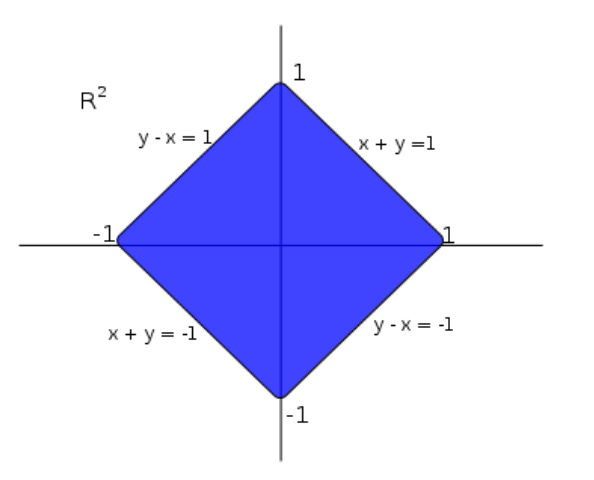
\includegraphics[width=6cm]{week1/f_1_1}
\caption{$B_1(\bm0)$ w.r.t. the metric $d_1$}
\end{figure}
\begin{figure}[H]
\centering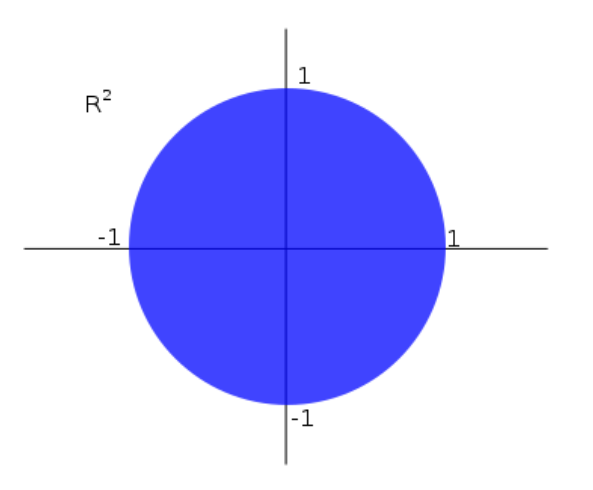
\includegraphics[width=6cm]{week1/f_1_2}
\caption{$B_1(\bm0)$ w.r.t. the metric $d_2$}
\end{figure}
\end{enumerate}
\end{example}













